\documentclass[12pt, oneside, titlepage]{article}   	% use "amsart" instead of "article" for AMSLaTeX format

\usepackage{graphicx}
\graphicspath{ {\string} }
\usepackage{subcaption}

%%%%%%%%%%%%%%%%%%%%%%%%%%%%%%%%%%%%%%%%%%%%%%%%%%%%
% set up packages
%%%%%%%%%%%%%%%%%%%%%%%%%%%%%%%%%%%%%%%%%%%%%%%%%%%%
\usepackage{geometry}                
\usepackage{textcomp}                
\usepackage{amsmath}                
\usepackage{graphicx}                
\usepackage{amssymb}                
\usepackage{fancyhdr}                
\usepackage{subcaption}                
\usepackage{bm}                
\usepackage{lineno}
% package for comments
\usepackage{soul}

\usepackage[breaklinks=true]{hyperref}

\usepackage[superscript,noadjust]{cite} % puts dash in citations to abbreviate
\usepackage [autostyle, english = american]{csquotes} % sets US-style quotes

\usepackage{etoolbox} % block quotes

\usepackage{float}
\usepackage{color}

\usepackage{pgf}
\usepackage{tikz}
\usepackage{eqnarray}

\usepackage{listings} % code blocks
\usepackage{setspace}

\usepackage{lscape}

% tikz background
\usetikzlibrary{backgrounds, fit}


\usepackage{natbib}
%\bibliographystyle{abbrvnat}
\setcitestyle{authoryear,open={(},close={)}}

%%%%%%%%%%%%%%%%%%%%%%%%%%%%%%%%%%%%%%%%%%%%%%%%%%%%
% call packages
%%%%%%%%%%%%%%%%%%%%%%%%%%%%%%%%%%%%%%%%%%%%%%%%%%%%	
\geometry{letterpaper, marginparwidth=60pt} % sets up geometry              		
\linenumbers % adds line numbers 
\MakeOuterQuote{"} % sets quote style
\doublespacing % setspace

%%%%%%%%%%%%%%%%%%%%%%%%%%%%%%%%%%%%%%%%%%%%%%%%%%%%
% patches with etoolbox 
%%%%%%%%%%%%%%%%%%%%%%%%%%%%%%%%%%%%%%%%%%%%%%%%%%%%	
% block quotes
\AtBeginEnvironment{quote}{\small}

% linenumbers
\makeatletter
\patchcmd{\@startsection}{\@ifstar}{\nolinenumbers\@ifstar}{}{}
\patchcmd{\@xsect}{\ignorespaces}{\linenumbers\ignorespaces}{}{}
\makeatother

%%%%%%%%%%%%%%%%%%%%%%%%%%%%%%%%%%%%%%%%%%%%%%%%%%%%
% tikzlibrary modifications
%%%%%%%%%%%%%%%%%%%%%%%%%%%%%%%%%%%%%%%%%%%%%%%%%%%%	
\usetikzlibrary{fit}
\usetikzlibrary{positioning}
\usetikzlibrary{arrows}
\usetikzlibrary{automata}

%%%%%%%%%%%%%%%%%%%%%%%%%%%%%%%%%%%%%%%%%%%%%%%%%%%%
% page formatting; exact 1 in margins
%%%%%%%%%%%%%%%%%%%%%%%%%%%%%%%%%%%%%%%%%%%%%%%%%%%%
\pagestyle{plain}                                                     

\setlength{\textwidth}{6.5in}    
\setlength{\oddsidemargin}{0in}
\setlength{\evensidemargin}{0in}
\setlength{\textheight}{8.5in}
\setlength{\topmargin}{0in}
\setlength{\headheight}{0in}
\setlength{\headsep}{0in}
\setlength{\footskip}{.5in}

%%%%%%%%%%%%%%%%%%%%%%%%%%%%%%%%%%%%%%%%%%%%%%%%%%%%
% defining code blocks using listings package
%%%%%%%%%%%%%%%%%%%%%%%%%%%%%%%%%%%%%%%%%%%%%%%%%%%%

\definecolor{dkgreen}{rgb}{0,0.6,0}
\definecolor{gray}{rgb}{0.5,0.5,0.5}
\definecolor{mauve}{rgb}{0.58,0,0.82}

\lstset{frame=tb,
  language=R,
  aboveskip=3mm,
  belowskip=3mm,
  showstringspaces=false,
  columns=flexible,
  basicstyle={\small\ttfamily},
  numbers=none,
  numberstyle=\tiny\color{gray},
 % keywordstyle=\color{blue},
  commentstyle=\color{dkgreen},
  stringstyle=\color{mauve},
  breaklines=true,
  breakatwhitespace=true,
  tabsize=3,
  otherkeywords={0,1,2,3,4,5,6,7,8,9},
  deletekeywords={data,frame,length,as,character,dunif,ps},
}

%%%%%%%%%%%%%%%%%%%%%%%%%%%%%%%%%%%%%%%%%%%%%%%%%%%%
%%%%%%%%%%%%%%%%%%%%%%%%%%%%%%%%%%%%%%%%%%%%%%%%%%%%
% begin document
%%%%%%%%%%%%%%%%%%%%%%%%%%%%%%%%%%%%%%%%%%%%%%%%%%%%
%%%%%%%%%%%%%%%%%%%%%%%%%%%%%%%%%%%%%%%%%%%%%%%%%%%%

\begin{document}

Last updated: \today

\section{Appendix: Posteriors and joint likelihoods}

Add description of this appendix. The appendix includes directed acyclic graphs, and posterior and proportion joint distributions for all models.

\clearpage
\newpage

\section{Full model: germination, seed survivorship, initial seed survival}
%%%%%%%%%%%%%%%%%%%%%%%%%%%%%%%%%%%%%%%%%%%%%%%%%%%%
% DIRECTED ACYCLIC GRAPHS FOR SEED DECAY MODEL
%%%%%%%%%%%%%%%%%%%%%%%%%%%%%%%%%%%%%%%%%%%%%%%%%%%%
\begin{figure}[h]%
\begin{subfigure}[c]{\textwidth}
 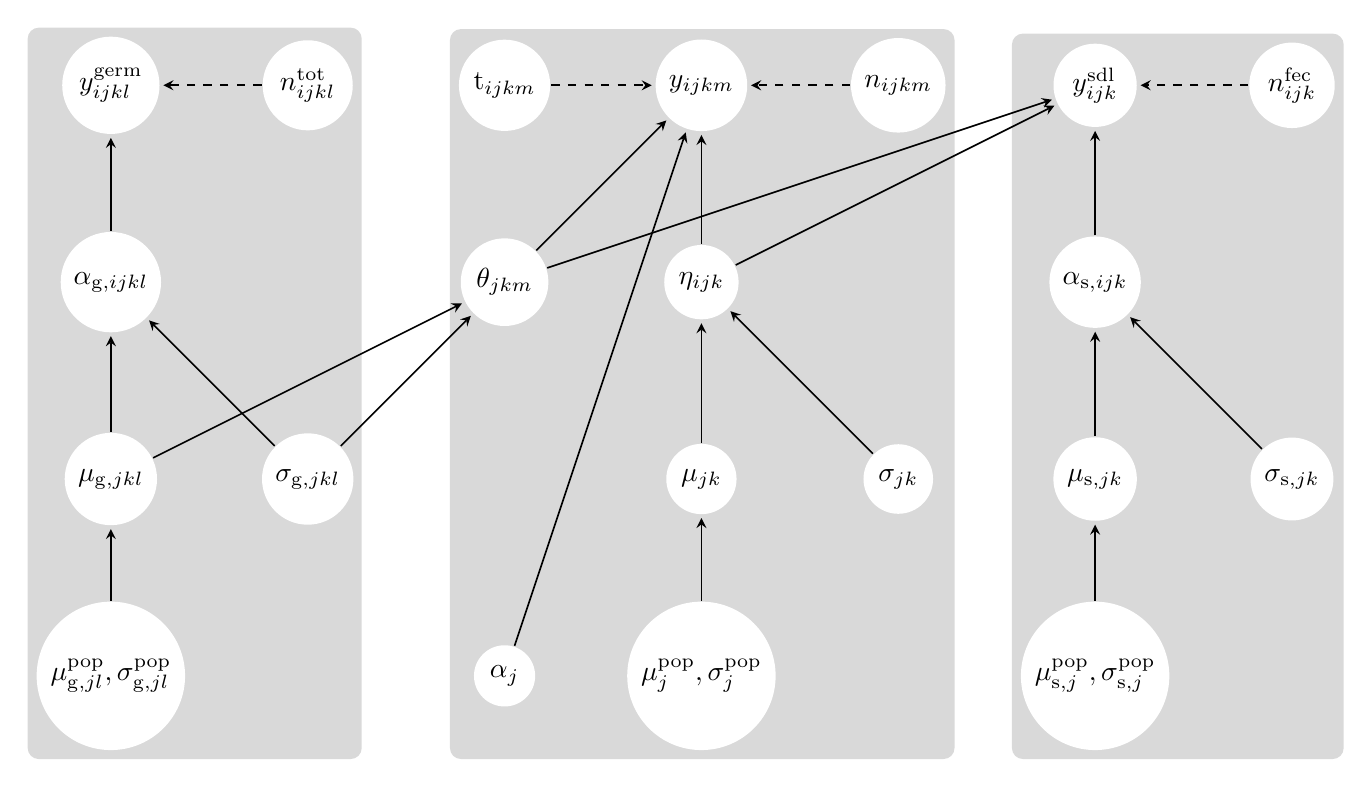
\begin{tikzpicture}[
            > = stealth, % arrow head style
            shorten > = 1pt, % don't touch arrow head to node
            auto,
            node distance = 2.5cm, % distance between nodes
            semithick % line style
        ]

        \tikzstyle{every state}=[
            draw = none,
            thick,
            fill = white,
            minimum size = 4mm
        ]


	% data level
        \node[state] (Y) [] {$y^{\mathrm{germ}}_{ijkl}$};
        \node[state] (N) [right of=Y] {$n^{\mathrm{tot}}_{ijkl}$};
       
        \path[dashed,->] (N) edge node {} (Y);
                  
         % hyperparameters
         \node[state] (AB) [below of = Y] {$\alpha_{\mathrm{g},ijkl}$};
                
         \path[->] (AB) edge node {} (Y);
         
          % hyperparameters
        
         \node[state] (MS) [below of = AB] {$\mu_{\mathrm{g},jkl}$};
         \node[state] (A)[ right of = MS]  {$\sigma_{\mathrm{g},jkl}$};
         
         \path[->] (A) edge node {} (AB);       
         \path[->] (MS) edge node {} (AB);       
         
         \node[state] (H) [below of = MS] {$\mu^\mathrm{pop}_{\mathrm{g},jl},\sigma^\mathrm{pop}_{\mathrm{g},jl}$};
         \path[->] (H) edge node {} (MS);       
          
         %% SURVIVAL

	% data level
        \node[state] (T2) [right of = N] {$\mathrm{t}_{ijkm}$};
        \node[state] (Y2) [right of = T2] {$y_{ijkm}$};
        \node[state] (N2) [right of=Y2] {$n_{ijkm}$};

        \path[dashed,->] (N2) edge node {} (Y2);

        \path[dashed,->] (T2) edge node {} (Y2);

                  % hyperparameters
        \node[state] (AB2) [below of = Y2] {$\eta_{ijk}$};
       \node[state] (TH2) [left of = AB2] {$\theta_{jkm}$};
        
         \path[->] (AB2) edge node {} (Y2);
         \path[->] (TH2) edge node {} (Y2);
         \path[->] (MS) edge node {} (TH2);
          \path[->] (A) edge node {} (TH2);
                  
          % hyperparameters
        
         \node[state] (MS2) [below of = AB2] {$\mu_{jk}$};
         \node[state] (A2) [ right of = MS2]  {$\sigma_{jk}$};
         
         \path[->] (A2) edge node {} (AB2);       
         \path[->] (MS2) edge node {} (AB2);       
         
         \node[state] (H2) [below of = MS2] {$\mu^\mathrm{pop}_{j},\sigma^\mathrm{pop}_{j}$};
         \path[->] (H2) edge node {} (MS2);       
         
         \node[state] (ALPHA2) [left of = H2] {$\alpha_{j}$};
         \path[->] (ALPHA2) edge node {} (Y2);       

         % INITIAL SURVIVAL

	% data level
        \node[state] (Y3) [right of =N2] {$y^{\mathrm{sdl}}_{ijk}$};
        \node[state] (N3) [right of=Y3] {$n^{\mathrm{fec}}_{ijk}$};
       
        \path[dashed,->] (N3) edge node {} (Y3);
                   
        % hyperparameters
         \node[state] (AB3) [below of = Y3] {$\alpha_{\mathrm{s},ijk}$};
               
         \path[->] (AB3) edge node {} (Y3);
         \path[->] (AB2) edge node {} (Y3);
         \path[->] (TH2) edge node {} (Y3);
        
          % hyperparameters
        
         \node[state] (MS3) [below of = AB3] {$\mu_{\mathrm{s},jk}$};
         \node[state] (A3)[ right of = MS3]  {$\sigma_{\mathrm{s},jk}$};
         
         \path[->] (A3) edge node {} (AB3);       
         \path[->] (MS3) edge node {} (AB3);       
         
         \node[state] (H3) [below of = MS3] {$\mu^\mathrm{pop}_{\mathrm{s},j},\sigma^\mathrm{pop}_{\mathrm{s},j}$};
         \path[->] (H3) edge node {} (MS3);       
         
         
         % BACKGROUND


          \begin{scope}[on background layer]
   \node [fit=(T2) (N2) (H2), fill= gray!30, rounded corners, inner sep=.1cm] {};
   \node [fit=(Y) (N) (H), fill= gray!30, rounded corners, inner sep=.1cm] {};
   \node [fit=(Y3) (N3) (H3), fill= gray!30, rounded corners, inner sep=.1cm] {};
  \end{scope}
                   
  \end{tikzpicture}
\subcaption{Directed acyclic graphs for the joint models for seed germination, persistence, and survival from seed production to the first October. Solid arrows depict the relationships among random variables, and dashed arrows depict the deterministic relationships.}
\end{subfigure}
\end{figure}

%%%%%%%%%%%%%%%%%%%%%%%%%%%%%%%%%%%%%%%%%%%%%%%%%%%%
% POSTERIOR AND JOINT DISTRIBUTIONS FOR SEED BAG EXPERIMENT
%%%%%%%%%%%%%%%%%%%%%%%%%%%%%%%%%%%%%%%%%%%%%%%%%%%%

\begin{align}
  \begin{split}
%  \beta_{ijk} & = \exp({ - \frac{ \eta_{ijk} }{ \alpha_j }})
% \\ g( \eta_{ijk}, \theta_{jkm},  t_{ijkm} ) & = \theta_{jkm}  \times \exp(- (\frac{ t_{ijkm} }{\beta_{ijk}})^{\alpha_j}  ) \\
%  & =  \theta_{jkm}  \times \exp(- (\frac{ t_{ijkm} }{ \exp({ - \frac{ \eta_{ijk} }{ \alpha_j}}) })^{\alpha_j}  ) 
& g( \eta_{ijk}, \theta_{jkm},  t_{ijkm} )  = \theta_{jkm}  \times \exp(- (\frac{ t_{ijkm} }{ \exp({ - \frac{ \eta_{ijk} }{ \alpha_j}}) })^{\alpha_j}  ) 
 \\  [ \bm{\mu}_\mathrm{g} , \bm{\sigma}_\mathrm{g} , & \bm{\mu}_\mathrm{g}^\mathrm{pop}, \bm{\sigma}_\mathrm{g}^\mathrm{pop} , \bm{\eta} , \bm{\mu} , \bm{\sigma} , \bm{\mu}^\mathrm{pop}, \bm{\sigma}^\mathrm{pop} |  \bm{\mathrm{y}}_\mathrm{g}, \bm{\mathrm{y}}  ]  \propto 
 \\ &   \prod_{i=1}^{I}  \prod_{j=1}^{J} \prod_{k=1}^{K} \Bigg[ \Big[ \prod_{m=1}^{M} 
   \mathrm{binomial} ( y_{ijkm} | n_{ijkm}, g( \theta_{jkm}, \eta_{ijk}, \alpha_j , t_{ijkm} ) ) 
   \\ & \times \mathrm{normal} ( \eta_{ijk}  | \mu_{jk}, \sigma{_{jk} })
  \\ & \times \mathrm{normal} ( \mu_{jk}  | \mu^\mathrm{pop}_{j}, \sigma^\mathrm{pop}_{j} ) \textrm{half-normal} ( \sigma_{jk} | 0,1)
  \\ & \times \mathrm{normal} ( \mu^\mathrm{pop}_{j} | 0 , 1 ) \textrm{half-normal} ( \sigma^\mathrm{pop}_{j} | 0,1)
  \\ & \times \mathrm{gamma} ( \alpha_j | 2 , 2 ) \Big]
  \\ & \Big[ \times \prod_{l=1}^{L} 
   \mathrm{binomial} ( y_{\mathrm{g},ijkl} | n_{\mathrm{g},ijkl}, \mathrm{logit}^{-1}(\alpha_{\mathrm{g},ijkl}) ) 
   \\ & \times \mathrm{normal} ( \alpha_{\mathrm{g},ijkl}  | \mu_{\mathrm{g},jkl}, \sigma{_{\mathrm{g},jkl} })
  \\ & \times \mathrm{normal} ( \mu_{\mathrm{g},jkl}  | \mu^\mathrm{pop}_{\mathrm{g},jl}, \sigma^\mathrm{pop}_{\mathrm{g},jl} ) \textrm{half-normal} ( \sigma_{\mathrm{g},jkl} | 0,1)
  \\ & \times \mathrm{normal} ( \mu^\mathrm{pop}_{\mathrm{g},jl} | 0 , 1 ) \textrm{half-normal} ( \sigma^\mathrm{pop}_{\mathrm{g},jl} | 0,1). \Big] \Bigg] 
  \\ & \prod_{i=1}^{I} \prod_{j=1}^{J} \prod_{k=2}^{K} \mathrm{binomial} ( y_{\mathrm{p},ijk} | n_{\mathrm{p},ijk}, g( \theta_{jk,m=1}, \eta_{ijk}, \alpha_j , t_{ijk,m=1} )  \mathrm{logit}^{-1}(\alpha_{\mathrm{s},ijk})  )
             \\ & \times \mathrm{normal} ( \alpha_{\mathrm{s},ijk}  | \mu_{\mathrm{g},jk}, \sigma{_{\mathrm{s},jk} })
  \\ & \times \mathrm{normal} ( \mu_{\mathrm{s},jk}  | \mu^\mathrm{pop}_{\mathrm{s},j}, \sigma^\mathrm{pop}_{\mathrm{s},j} )
  \\ & \times \textrm{half-normal} ( \sigma_{\mathrm{s},jk} | 0,1)
  \\ & \times \mathrm{normal} ( \mu^\mathrm{pop}_{\mathrm{s},j} | 0 , 1 ) \textrm{half-normal} ( \sigma^\mathrm{pop}_{\mathrm{s},j} | 0,1)
  \end{split}
\end{align}

\clearpage
\newpage

\subsection*{Viability trials}

%%%%%%%%%%%%%%%%%%%%%%%%%%%%%%%%%%%%%%%%%%%%%%%%%%%%
% DIRECTED ACYCLIC GRAPHS FOR VIABILITY TRIALS
%%%%%%%%%%%%%%%%%%%%%%%%%%%%%%%%%%%%%%%%%%%%%%%%%%%%

\begin{figure}[h]%
\begin{subfigure}[c]{\textwidth}
\centering
   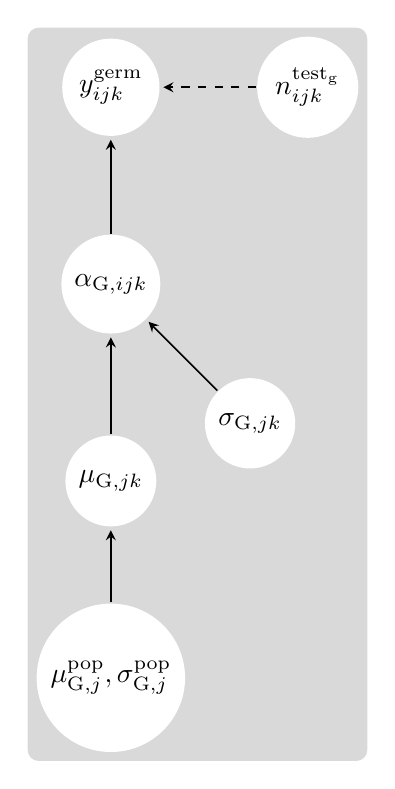
\begin{tikzpicture}[
            > = stealth, % arrow head style
            shorten > = 1pt, % don't touch arrow head to node
            auto,
            node distance = 2.5cm, % distance between nodes
            semithick % line style
        ]

        \tikzstyle{every state}=[
            draw = none,
            thick,
            fill = white,
            minimum size = 4mm
        ]F


	% data level
        \node[state] (Y) [] {$y^{\mathrm{germ}}_{ijk}$};
        \node[state] (N) [right of=Y] {$n^\mathrm{test_g}_{ijk}$};
       
        \path[dashed,->] (N) edge node {} (Y);

        % probability
        % \node[state] (T) [below of = Y] {$\theta_{ijk}$};
        %       
        % \path[->] (T) edge node {} (Y);
                  
                  % hyperparameters
         \node[state] (AB) [below of = Y] {$\alpha_{\mathrm{G},ijk}$};
                
         \path[->] (AB) edge node {} (Y);
         
          % hyperparameters
        
         \node[state] (MS) [below of = AB] {$\mu_{\mathrm{G},jk}$};
         \node[state] (A) [below right of = AB] {$\sigma_{\mathrm{G},jk}$};
         
         \path[->] (A) edge node {} (AB);       
         \path[->] (MS) edge node {} (AB);       
         
         \node[state] (H) [below of = MS] {$\mu^\mathrm{pop}_{\mathrm{G},j},\sigma^\mathrm{pop}_{\mathrm{G},j}$};
         \path[->] (H) edge node {} (MS);       

                    \begin{scope}[on background layer]
   \node [fit=(Y) (N) (H), fill= gray!30, rounded corners, inner sep=.1cm] {};
  \end{scope}
  
  \end{tikzpicture}
  %
    \hspace{1cm}% NO SPACE!
  % BEGIN FIGURE 3
   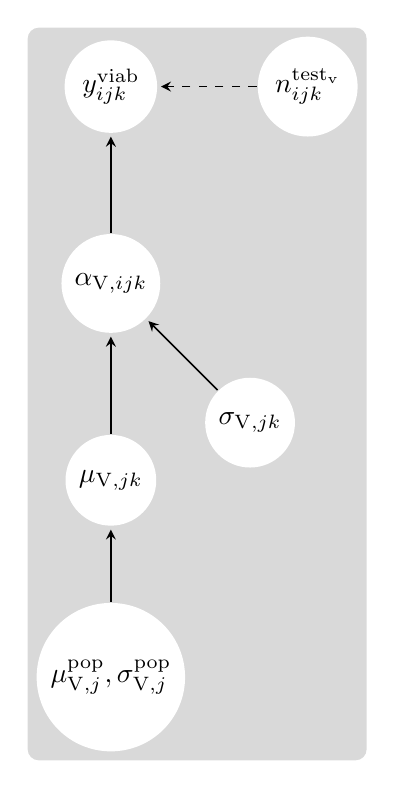
\begin{tikzpicture}[
            > = stealth, % arrow head style
            shorten > = 1pt, % don't touch arrow head to node
            auto,
            node distance = 2.5cm, % distance between nodes
            semithick % line style
        ]

        \tikzstyle{every state}=[
            draw = none,
            thick,
            fill = white,
            minimum size = 4mm
        ]F


	% data level
        \node[state] (Y) [] {$y^{\mathrm{viab}}_{ijk}$};
        \node[state] (N) [right of=Y] {$n^\mathrm{test_v}_{ijk}$};
       
        \path[dashed,->] (N) edge node {} (Y);

        % probability
        % \node[state] (T) [below of = Y] {$\theta_{ijk}$};
        %       
        % \path[->] (T) edge node {} (Y);
                  
                  % hyperparameters
         \node[state] (AB) [below of = Y] {$\alpha_{\mathrm{V},ijk}$};
                
         \path[->] (AB) edge node {} (Y);
         
          % hyperparameters
        
         \node[state] (MS) [below of = AB] {$\mu_{\mathrm{V},jk}$};
         \node[state] (A) [below right of = AB] {$\sigma_{\mathrm{V},jk}$};
         
         \path[->] (A) edge node {} (AB);       
         \path[->] (MS) edge node {} (AB);       
         
         \node[state] (H) [below of = MS] {$\mu^\mathrm{pop}_{\mathrm{V},j},\sigma^\mathrm{pop}_{\mathrm{V},j}$};
         \path[->] (H) edge node {} (MS);      
         
                             \begin{scope}[on background layer]
   \node [fit=(Y) (N) (H), fill= gray!30, rounded corners, inner sep=.1cm] {};
  \end{scope}
                                
  \end{tikzpicture}
\subcaption{Directed acyclic graphs for the hierarchical models for viability trials. Solid arrows depict the relationships among random variables, and dashed arrows depict the deterministic relationships.}
\end{subfigure}
\end{figure}
%
%%%%%%%%%%%%%%%%%%%%%%%%%%%%%%%%%%%%%%%%%%%%%%%%%%%%
% POSTERIOR AND JOINT DISTRIBUTIONS FOR VIABILITY TRIALS
%%%%%%%%%%%%%%%%%%%%%%%%%%%%%%%%%%%%%%%%%%%%%%%%%%%%

% QUESTIONS
% do I need to include \bm{n} on the RHS of the conditional statement for the posterior?


\begin{align}
  \begin{split}
 [  \bm{\alpha_G} , \bm{\mu_G} , \bm{\sigma_G} , \bm{\mu^\mathrm{pop}_G}, \bm{\sigma^\mathrm{pop}_G} | & \bm{y^{\mathrm{tot}}}  ] \propto \prod_{i=1}^{I}   \prod_{j=1}^{J}  \prod_{k=1}^{K} 
   \mathrm{binomial} ( y^{\mathrm{germ}}_{ijk} | n^\mathrm{test_g}_{ijk}, \mathrm{logit}^{-1}( \alpha_{G,ijk} ) ) 
   \\ & \times \mathrm{normal} ( \alpha_{G,ijk}  | \mu_{G,jk}, \sigma{_{G,jk} })
  \\ & \times \mathrm{normal} ( \mu_{G,jk}  | \mu^\mathrm{pop}_{G,j}, \sigma^\mathrm{pop}_{G,j} )
  \\ & \times \textrm{half-normal} ( \sigma_{G,jk} | 0,1)
  \\ & \times \mathrm{normal} ( \mu^\mathrm{pop}_{G,j} | 0 , 1 ) \textrm{half-normal} ( \sigma^\mathrm{pop}_{G,j} | 0,1).
  \end{split}
\end{align}
%
\begin{align}
  \begin{split}
 [  \bm{\alpha_V} , \bm{\mu_V} , \bm{\sigma_V} , \bm{\mu^\mathrm{pop}_V}, \bm{\sigma^\mathrm{pop}_V} | & \bm{y^{\mathrm{tot}}}  ] \propto \prod_{i=1}^{I}   \prod_{j=1}^{J}  \prod_{k=1}^{K} 
   \mathrm{binomial} ( y^{\mathrm{viab}}_{ijk} | n^\mathrm{test_v}_{ijk}, \mathrm{logit}^{-1}( \alpha_{V,ijk} ) ) 
   \\ & \times \mathrm{normal} ( \alpha_{V,ijk}  | \mu_{V,jk}, \sigma{_{V,jk} })
  \\ & \times \mathrm{normal} ( \mu_{V,jk}  | \mu^\mathrm{pop}_{V,j}, \sigma^\mathrm{pop}_{V,j} )
  \\ & \times \textrm{half-normal} ( \sigma_{V,jk} | 0,1)
  \\ & \times \mathrm{normal} ( \mu^\mathrm{pop}_{V,j} | 0 , 1 ) \textrm{half-normal} ( \sigma^\mathrm{pop}_{V,j} | 0,1).
  \end{split}
\end{align}
%

\clearpage
\newpage

\subsection*{Survival of seedlings to fruiting plants}

%%%%%%%%%%%%%%%%%%%%%%%%%%%%%%%%%%%%%%%%%%%%%%%%%%%%
% DIRECTED ACYCLIC GRAPHS FOR SEED SURVIVAL
%%%%%%%%%%%%%%%%%%%%%%%%%%%%%%%%%%%%%%%%%%%%%%%%%%%%
\begin{figure}[!h]%
\begin{subfigure}[c]{\textwidth}
\centering
   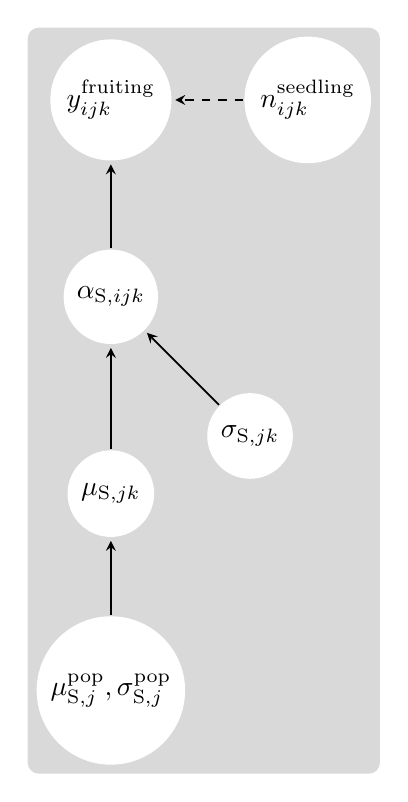
\begin{tikzpicture}[
            > = stealth, % arrow head style
            shorten > = 1pt, % don't touch arrow head to node
            auto,
            node distance = 2.5cm, % distance between nodes
            semithick % line style
        ]

        \tikzstyle{every state}=[
            draw = none,
            thick,
            fill = white,
            minimum size = 4mm
        ]F
% data level
        \node[state] (Y) [] {$y^{\mathrm{fruiting}}_{ijk}$};
        \node[state] (N) [right of=Y] {$n^\mathrm{seedling}_{ijk}$};
       
        \path[dashed,->] (N) edge node {} (Y);

        % probability
        % \node[state] (T) [below of = Y] {$\theta_{ijk}$};
        %       
        % \path[->] (T) edge node {} (Y);
                  
                  % hyperparameters
         \node[state] (AB) [below of = Y] {$\alpha_{\mathrm{S},ijk}$};
                
         \path[->] (AB) edge node {} (Y);
         
          % hyperparameters
        
         \node[state] (MS) [below of = AB] {$\mu_{\mathrm{S},jk}$};
         \node[state] (A) [below right of = AB] {$\sigma_{\mathrm{S},jk}$};
         
         \path[->] (A) edge node {} (AB);       
         \path[->] (MS) edge node {} (AB);       
         
         \node[state] (H) [below of = MS] {$\mu^\mathrm{pop}_{\mathrm{S},j},\sigma^\mathrm{pop}_{\mathrm{S},j}$};
         \path[->] (H) edge node {} (MS);       

                    \begin{scope}[on background layer]
   \node [fit=(Y) (N) (H), fill= gray!30, rounded corners, inner sep=.1cm] {};
  \end{scope}
  
  \end{tikzpicture}

\subcaption{Directed acyclic graphs for the hierarchical models for seedling survival to fruiting. Solid arrows depict the relationships among random variables, and dashed arrows depict the deterministic relationships.}
\end{subfigure}
\end{figure}

%
%%%%%%%%%%%%%%%%%%%%%%%%%%%%%%%%%%%%%%%%%%%%%%%%%%%%
% POSTERIOR AND JOINT DISTRIBUTIONS FOR SEED SURVIVAL
%%%%%%%%%%%%%%%%%%%%%%%%%%%%%%%%%%%%%%%%%%%%%%%%%%%%

% QUESTIONS
% do I need to include \bm{n} on the RHS of the conditional statement for the posterior?

\begin{align}
  \begin{split}
 [  \bm{\alpha_S} , \bm{\mu_S} , \bm{\sigma_S} , \bm{\mu^\mathrm{pop}_S}, \bm{\sigma^\mathrm{pop}_S} | & \bm{y^{\mathrm{fruiting}}}  ] \propto \prod_{i=1}^{I}   \prod_{j=1}^{J}  \prod_{k=1}^{K} 
   \mathrm{binomial} ( y^{\mathrm{fruiting}}_{ijk} | n^\mathrm{seedling}_{ijk}, \mathrm{logit}^{-1}( \alpha_{S,ijk} ) ) 
   \\ & \times \mathrm{normal} ( \alpha_{S,ijk}  | \mu_{S,jk}, \sigma{_{S,jk} })
  \\ & \times \mathrm{normal} ( \mu_{S,jk}  | \mu^\mathrm{pop}_{S,j}, \sigma^\mathrm{pop}_{S,j} )
  \\ & \times \textrm{half-normal} ( \sigma_{S,jk} | 0,1)
  \\ & \times \mathrm{normal} ( \mu^\mathrm{pop}_{S,j} | 0 , 1 ) \textrm{half-normal} ( \sigma^\mathrm{pop}_{S,j} | 0,1).
  \end{split}
\end{align}


\clearpage
\newpage

\subsection*{Fruits per plant and seeds per fruit}

%%%%%%%%%%%%%%%%%%%%%%%%%%%%%%%%%%%%%%%%%%%%%%%%%%%%
% DIRECTED ACYCLIC GRAPHS FOR FECUNDITY
%%%%%%%%%%%%%%%%%%%%%%%%%%%%%%%%%%%%%%%%%%%%%%%%%%%%
\begin{figure}[h]%
\begin{subfigure}[c]{\textwidth}
\centering
   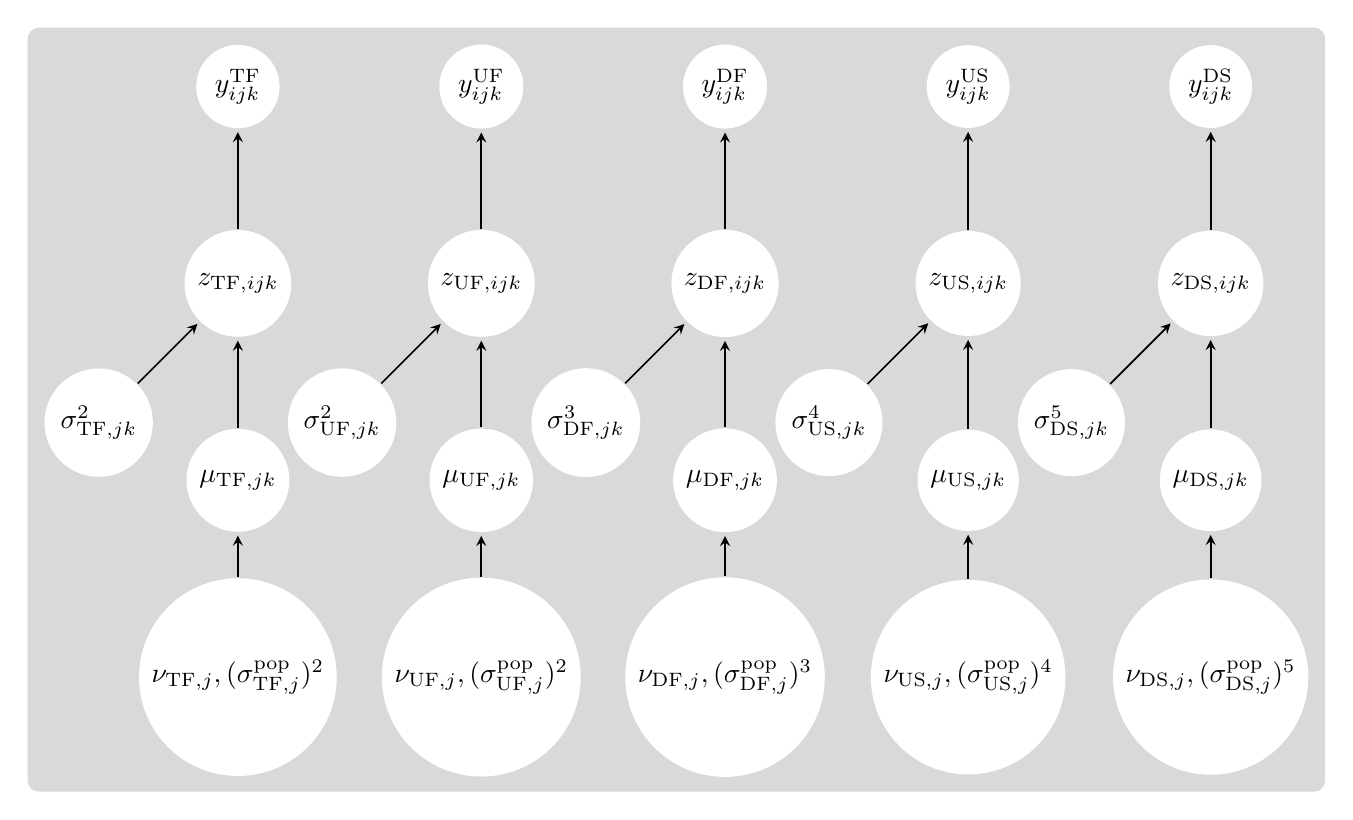
\begin{tikzpicture}[
            > = stealth, % arrow head style
            shorten > = 1pt, % don't touch arrow head to node
            auto,
            node distance = 2.5cm, % distance between nodes
            semithick % line style
            ]

        \tikzstyle{every state}=[
            draw = none,
            thick,
            fill = white,
            minimum size = 4mm
        ]F


	% data level
	\node[state] (Y) [] {$y^{\mathrm{UF}}_{ijk}$};
	\node[state] (Y2) [left =2cm of Y] {$y^{\mathrm{TF}}_{ijk}$};
       	\node[state] (Y3) [right  =2cm of Y] {$y^{\mathrm{DF}}_{ijk}$};
         \node[state] (Y4) [right  =2cm of Y3] {$y^{\mathrm{US}}_{ijk}$};
         \node[state] (Y5) [right  =2cm of Y4] {$y^{\mathrm{DS}}_{ijk}$};
    

        
        % parameters
         \node[state] (A) [below of = Y] {$z_{\mathrm{UF},ijk}$};          
         \path[->] (A) edge node {} (Y);
         
          \node[state] (MU) [below of = A] {$\mu_{\mathrm{UF},jk}$};
         \node[state] (SIG) [below left of = A] {$\sigma_{\mathrm{UF},jk}^2$};
         
         \path[->] (SIG) edge node {} (A);       
         \path[->] (MU) edge node {} (A);       
         
         \node[state] (H) [below of = MU] {$\nu_{\mathrm{UF},j},(\sigma^\mathrm{pop}_{\mathrm{UF},j})^2$};
         \path[->] (H) edge node {} (MU);       
         
         
         % parameters
         \node[state] (A2) [below of = Y2] {$z_{\mathrm{TF},ijk}$};          
         \path[->] (A2) edge node {} (Y2);
         
          \node[state] (MU2) [below of = A2] {$\mu_{\mathrm{TF},jk}$};
         \node[state] (SIG2) [below left of = A2] {$\sigma_{\mathrm{TF},jk}^2$};
         
         \path[->] (SIG2) edge node {} (A2);       
         \path[->] (MU2) edge node {} (A2);       
         
         \node[state] (H2) [below of = MU2] {$\nu_{\mathrm{TF},j},(\sigma^\mathrm{pop}_{\mathrm{TF},j})^2$};
         \path[->] (H2) edge node {} (MU2);       

         % parameters
         \node[state] (A3) [below of = Y3] {$z_{\mathrm{DF},ijk}$};          
         \path[->] (A3) edge node {} (Y3);
         
          \node[state] (MU3) [below of = A3] {$\mu_{\mathrm{DF},jk}$};
         \node[state] (SIG3) [below left of = A3] {$\sigma_{\mathrm{DF},jk}^3$};
         
         \path[->] (SIG3) edge node {} (A3);       
         \path[->] (MU3) edge node {} (A3);       
         
         \node[state] (H3) [below of = MU3] {$\nu_{\mathrm{DF},j},(\sigma^\mathrm{pop}_{\mathrm{DF},j})^3$};
         \path[->] (H3) edge node {} (MU3);      

                   % parameters
         \node[state] (A4) [below of = Y4] {$z_{\mathrm{US},ijk}$};          
         \path[->] (A4) edge node {} (Y4);
         
          \node[state] (MU4) [below of = A4] {$\mu_{\mathrm{US},jk}$};
         \node[state] (SIG4) [below left of = A4] {$\sigma_{\mathrm{US},jk}^4$};
         
         \path[->] (SIG4) edge node {} (A4);       
         \path[->] (MU4) edge node {} (A4);       
         
         \node[state] (H4) [below of = MU4] {$\nu_{\mathrm{US},j},(\sigma^\mathrm{pop}_{\mathrm{US},j})^4$};
         \path[->] (H4) edge node {} (MU4);      
         
                  % parameters
         \node[state] (A5) [below of = Y5] {$z_{\mathrm{DS},ijk}$};          
         \path[->] (A5) edge node {} (Y5);
         
          \node[state] (MU5) [below of = A5] {$\mu_{\mathrm{DS},jk}$};
         \node[state] (SIG5) [below left of = A5] {$\sigma_{\mathrm{DS},jk}^5$};
         
         \path[->] (SIG5) edge node {} (A5);       
         \path[->] (MU5) edge node {} (A5);       
         
         \node[state] (H5) [below of = MU5] {$\nu_{\mathrm{DS},j},(\sigma^\mathrm{pop}_{\mathrm{DS},j})^5$};
         \path[->] (H5) edge node {} (MU5);      
                                           
          \begin{scope}[on background layer]
   \node [fit=(SIG2) (Y) (H5), fill= gray!30, rounded corners, inner sep=.2cm] {};
 \end{scope}
                                 
  \end{tikzpicture}
\subcaption{Directed acyclic graphs for the hierarchical models fruits per plant and seeds per fruit. Solid arrows depict the relationships among random variables, and dashed arrows depict the deterministic relationships.}
\end{subfigure}
\end{figure}

%
%%%%%%%%%%%%%%%%%%%%%%%%%%%%%%%%%%%%%%%%%%%%%%%%%%%%
% POSTERIOR AND JOINT DISTRIBUTIONS FOR FECUNDITY
%%%%%%%%%%%%%%%%%%%%%%%%%%%%%%%%%%%%%%%%%%%%%%%%%%%%

% QUESTIONS
% do I need to include \bm{n} on the RHS of the conditional statement for the posterior?

\begin{align}
  \begin{split}
  & g( \theta )  = \exp{\theta}
 \\ [ &  \bm{z_{\mathrm{TF}}} ,  \bm{z_{\mathrm{UF}}},  \bm{z_{\mathrm{DF}}},  \bm{z_{\mathrm{US}}},  \bm{z_{\mathrm{DS}}},  \bm{\mu_{\mathrm{TF}}} ,  \bm{\mu_{\mathrm{UF}}},  \bm{\mu_{\mathrm{DF}}},  \bm{\mu_{\mathrm{US}}},  \bm{\mu_{\mathrm{DS}}},   \bm{\sigma_{\mathrm{TF}}}^2 ,  \bm{\sigma_{\mathrm{UF}}}^2,  \bm{\sigma_{\mathrm{DF}}}^2,  \bm{\sigma_{\mathrm{US}}}^2,  \bm{\sigma_{\mathrm{DS}}}^2, \\ & ( \bm{\sigma^\mathrm{pop}_{\mathrm{TF}}})^2, ( \bm{\sigma^\mathrm{pop}_{\mathrm{UF}}})^2, ( \bm{\sigma^\mathrm{pop}_{\mathrm{DF}}})^2, ( \bm{\sigma^\mathrm{pop}_{\mathrm{US}}})^2, ( \bm{\sigma^\mathrm{pop}_{\mathrm{DS}}})^2,  \bm{\nu_{\mathrm{TF}}} ,  \bm{\nu_{\mathrm{UF}}},  \bm{\nu_{\mathrm{DF}}},  \bm{\nu_{\mathrm{US}}},  \bm{\nu_{\mathrm{DS}}}, |  \bm{y^{\mathrm{TF}}} , \bm{y^{\mathrm{UF}}} , \bm{y^{\mathrm{DF}}} , \bm{y^{\mathrm{US}}} , \bm{y^{\mathrm{DS}}} ]  \propto  \\  
 	     & \prod_{j=1}^{J}  \Big\{ \prod_{i=1}^{N_1}  \prod_{k=1}^{K_1}  \mathrm{Poisson} ( y^\mathrm{TF}_{ijk} | z_{\mathrm{TF},ijk} )\ \mathrm{lognormal} ( z_{\mathrm{TF},ijk} | \mathrm{log}(\mu_{\mathrm{TF},jk}), \sigma^2_{\mathrm{TF},jk} )  \\
	     & \times \mathrm{lognormal} ( \mu_{\mathrm{TF},jk} | \mathrm{log}(\mathrm{g}(\nu_{\mathrm{TF},j}), (\sigma^\mathrm{pop}_{\mathrm{TF},j} )^2)  \\
	     & \times \textrm{half-normal}  ( \sigma^2_{\mathrm{TF},jk}  | 0, 1 ) \\
	     & \times \mathrm{gamma} (\nu_{\mathrm{TF},j} | 1 , 1)\  \textrm{half-normal} ( (\sigma^\mathrm{pop}_{\mathrm{TF},j} )^2 | 0, 1 ) \Big\}  \\
  \times &  \Big\{ \prod_{i=1}^{N_2}  \prod_{k=1}^{K_2}  \mathrm{Poisson} ( y^\mathrm{UF}_{ijk} | z_{\mathrm{UF},ijk} )\  \mathrm{Poisson} ( y^\mathrm{DF}_{ijk} | z_{\mathrm{DF},ijk} ) \\
  & \times  \mathrm{lognormal} ( z_{\mathrm{UF},ijk} | \mathrm{log}(\mu_{\mathrm{UF},jk}), \sigma^2_{\mathrm{UF},jk} )\ \mathrm{lognormal} ( z_{\mathrm{DF},ijk} | \mathrm{log}(\mu_{\mathrm{DF},jk}), \sigma^2_{\mathrm{DF},jk} )    \\
	     & \times \mathrm{lognormal} ( \mu_{\mathrm{UF},jk} | \mathrm{log}(\mathrm{g}(\nu_{\mathrm{UF},j}), (\sigma^\mathrm{pop}_{\mathrm{UF},j} )^2 )\  \mathrm{lognormal} ( \mu_{\mathrm{DF},jk} | \mathrm{log}(\mathrm{g}(\nu_{\mathrm{DF},j}), (\sigma^\mathrm{pop}_{\mathrm{DF},j} )^2 )   \\
	     & \times \textrm{half-normal}  ( \sigma^2_{\mathrm{UF},jk}  | 0, 1 )\ \textrm{half-normal}  ( \sigma^2_{\mathrm{DF},jk}  | 0, 1 ) \\
	     & \times \mathrm{gamma} (\nu_{\mathrm{UF},j} | 1 , 1)\  \textrm{half-normal} ( (\sigma^\mathrm{pop}_{\mathrm{UF},j} )^2  | 0, 1 ) \\
	     & \times  \mathrm{gamma} (\nu_{\mathrm{DF},j} | 1 , 1)\  \textrm{half-normal} ( (\sigma^\mathrm{pop}_{\mathrm{DF},j} )^2  | 0, 1 ) \Big\}  \\
	      & \times \Big\{  \prod_{i=1}^{N_3}  \prod_{k=1}^{K_3}  \mathrm{Poisson} ( y^\mathrm{US}_{ijk} | z_{\mathrm{US},ijk} )\ \mathrm{lognormal} ( z_{\mathrm{US},ijk} | \mathrm{log}(\mu_{\mathrm{UF},jk}), \sigma^2_{\mathrm{US},jk} )  \\
	     & \times \mathrm{lognormal} ( \mu_{\mathrm{US},jk} | \mathrm{log}(\mathrm{g}(\nu_{\mathrm{US},j}), (\sigma^\mathrm{pop}_{\mathrm{US},j} )^2 )  \\
	     & \times \textrm{half-normal} ( \sigma^2_{\mathrm{US},jk}  | 0, 1 ) \\
	     & \times \mathrm{gamma} (\nu_{\mathrm{US},j} | 1 , 1)\  \textrm{half-normal} ( (\sigma^\mathrm{pop}_{\mathrm{US},j} )^2  | 0, 1 ) \Big\}   \\
	     & \times \Big\{  \prod_{i=1}^{N_4}  \prod_{k=1}^{K_4}  \mathrm{Poisson} ( y^\mathrm{DS}_{ijk} | z_{\mathrm{DS},ijk} )\ \mathrm{lognormal} ( z_{\mathrm{DS},ijk} | \mathrm{log}(\mu_{\mathrm{UF},jk}), \sigma^2_{\mathrm{DS},jk} )  \\
	     & \times \mathrm{lognormal} ( \mu_{\mathrm{DS},jk} | \mathrm{log}(\mathrm{g}(\nu_{\mathrm{DS},j}), (\sigma^\mathrm{pop}_{\mathrm{DS},j} )^2 )  \\
	     & \times \textrm{half-normal}  ( \sigma^2_{\mathrm{DS},jk}  | 0, 1 ) \\
	     & \times \mathrm{gamma} (\nu_{\mathrm{DS},j} | 1 , 1)\  \textrm{half-normal} ( (\sigma^\mathrm{pop}_{\mathrm{DS},j} )^2  | 0,1) \Big\}.
  \end{split}
\end{align}



\iffalse
%%%%%%%%%%%%%%%%%%%%%%%%%%%%%%%%%%%%%%%%%%%%%%%%%%%%
% DIRECTED ACYCLIC GRAPHS FOR FECUNDITY
%%%%%%%%%%%%%%%%%%%%%%%%%%%%%%%%%%%%%%%%%%%%%%%%%%%%
\begin{figure}[h]%
\begin{subfigure}[c]{\textwidth}
\centering
   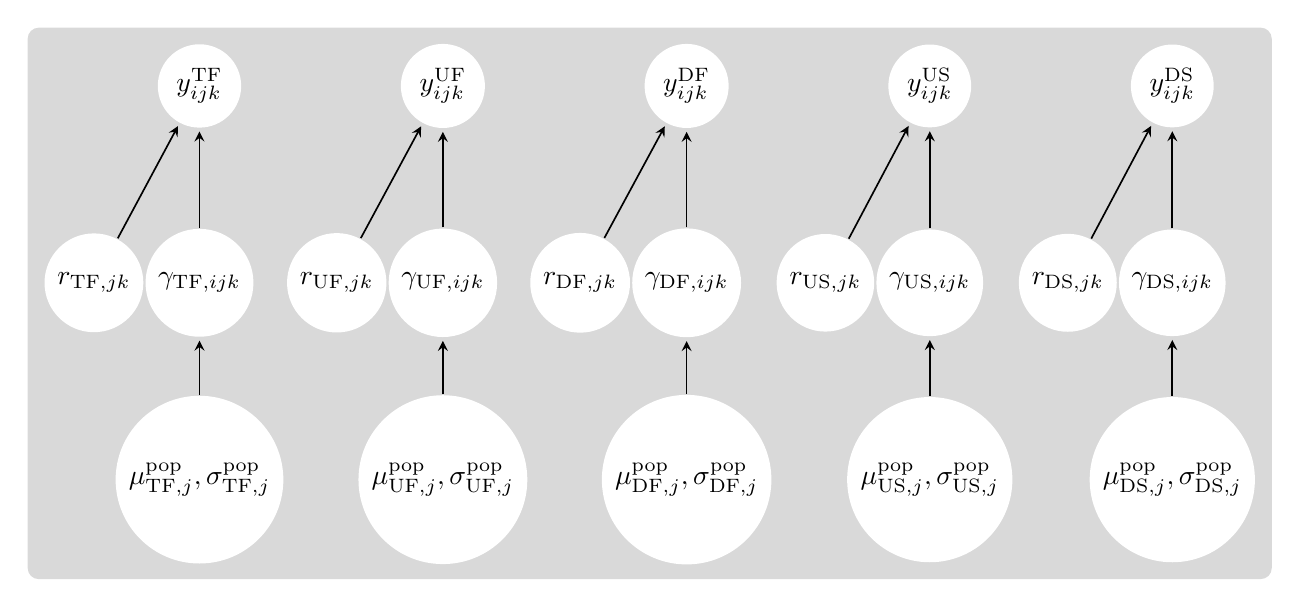
\begin{tikzpicture}[
            > = stealth, % arrow head style
            shorten > = 1pt, % don't touch arrow head to node
            auto,
            node distance = 2.5cm, % distance between nodes
            semithick % line style
            ]

        \tikzstyle{every state}=[
            draw = none,
            thick,
            fill = white,
            minimum size = 4mm
        ]F


	% data level
	\node[state] (Y) [] {$y^{\mathrm{UF}}_{ijk}$};
	\node[state] (Y2) [left =2cm of Y] {$y^{\mathrm{TF}}_{ijk}$};
       	\node[state] (Y3) [right  =2cm of Y] {$y^{\mathrm{DF}}_{ijk}$};
         \node[state] (Y4) [right  =2cm of Y3] {$y^{\mathrm{US}}_{ijk}$};
         \node[state] (Y5) [right  =2cm of Y4] {$y^{\mathrm{DS}}_{ijk}$};
    
        
        % rparameters
         \node[state] (A) [below of = Y] {$\gamma_{\mathrm{UF},ijk}$};  
         \path[->] (A) edge node {} (Y);
         \node[state] (B) [left = 0cm of A] {$r_{\mathrm{UF},jk}$};  
         \path[->] (B) edge node {} (Y);
               
         \node[state] (A2) [below of = Y2] {$\gamma_{\mathrm{TF},ijk}$};
         \path[->] (A2) edge node {} (Y2);
         \node[state] (B2) [left = 0cm of A2] {$r_{\mathrm{TF},jk}$};  
         \path[->] (B2) edge node {} (Y2);
                  
         \node[state] (A3) [below of = Y3] {$\gamma_{\mathrm{DF},ijk}$};
         \path[->] (A3) edge node {} (Y3);
         \node[state] (B3) [left = 0cm of A3] {$r_{\mathrm{DF},jk}$};  
         \path[->] (B3) edge node {} (Y3);
                  
                  \node[state] (A4) [below of = Y4] {$\gamma_{\mathrm{US},ijk}$};
         \path[->] (A4) edge node {} (Y4);
         \node[state] (B4) [left = 0cm of A4] {$r_{\mathrm{US},jk}$};  
         \path[->] (B4) edge node {} (Y4);
          
                   \node[state] (A5) [below of = Y5] {$\gamma_{\mathrm{DS},ijk}$};
         \path[->] (A5) edge node {} (Y5);           
         \node[state] (B5) [left = 0cm of A5] {$r_{\mathrm{DS},jk}$};  
         \path[->] (B5) edge node {} (Y5);
                     
          % hyperparameters
         \node[state] (C) [below of = A] {$\mu^\mathrm{pop}_{\mathrm{UF},j},\sigma^\mathrm{pop}_{\mathrm{UF},j}$};
         \path[->] (C) edge node {} (A);           
         
                  \node[state] (C2) [below of = A2] {$\mu^\mathrm{pop}_{\mathrm{TF},j},\sigma^\mathrm{pop}_{\mathrm{TF},j}$};
         \path[->] (C2) edge node {} (A2);         
         
                  \node[state] (C3) [below of = A3] {$\mu^\mathrm{pop}_{\mathrm{DF},j},\sigma^\mathrm{pop}_{\mathrm{DF},j}$};
         \path[->] (C3) edge node {} (A3);         
         
          \node[state] (C4) [below of = A4] {$\mu^\mathrm{pop}_{\mathrm{US},j},\sigma^\mathrm{pop}_{\mathrm{US},j}$};
         \path[->] (C4) edge node {} (A4);      

          \node[state] (C5) [below of = A5] {$\mu^\mathrm{pop}_{\mathrm{DS},j},\sigma^\mathrm{pop}_{\mathrm{DS},j}$};
         \path[->] (C5) edge node {} (A5);      
                                  
          \begin{scope}[on background layer]
   \node [fit=(B2) (Y5) (C5), fill= gray!30, rounded corners, inner sep=.2cm] {};
  \end{scope}
                                 
  \end{tikzpicture}
\subcaption{Directed acyclic graphs for the hierarchical models fruits per plant and seeds per fruit. Solid arrows depict the relationships among random variables, and dashed arrows depict the deterministic relationships.}
\end{subfigure}
\end{figure}

%
%%%%%%%%%%%%%%%%%%%%%%%%%%%%%%%%%%%%%%%%%%%%%%%%%%%%
% POSTERIOR AND JOINT DISTRIBUTIONS FOR FECUNDITY
%%%%%%%%%%%%%%%%%%%%%%%%%%%%%%%%%%%%%%%%%%%%%%%%%%%%

% QUESTIONS
% do I need to include \bm{n} on the RHS of the conditional statement for the posterior?

\begin{align}
  \begin{split}
  [  \bm{\alpha_\mathrm{D}} , &  \bm{\alpha_4}, \bm{\theta}, \bm{\mu_\mathrm{D}} , \bm{\sigma_\mathrm{D}} , \bm{\mu_4} , \bm{\sigma_4} , \bm{\mu^\mathrm{pop}_\mathrm{D}}, \bm{\sigma^\mathrm{pop}_\mathrm{D}} , \bm{\mu^\mathrm{pop}_4}, \bm{\sigma^\mathrm{pop}_4} | \bm{y^\mathrm{oct}} , \bm{y^\mathrm{tot_2}}  ]  \propto  \\  
 	     & \prod_{j=1}^{J} \bigg\{ \Big\{ \prod_{i=1}^{N_1}  \prod_{k=1}^{K_1} \mathrm{binomial} \big( y^{\mathrm{oct}}_{ijk} | n^\mathrm{age_1}_{ijk}, \mathrm{logit}^{-1}( \alpha_{\mathrm{D},ijk} ) \big) \\
	      \times & \mathrm{normal} ( \alpha_{\mathrm{D},ijk}  | \mu_{\mathrm{D},jk}, \sigma{_{\mathrm{D},jk} }) \mathrm{normal} ( \mu_{\mathrm{D},jk}  | \mu^\mathrm{pop}_{\mathrm{D},j}, \sigma^\mathrm{pop}_{\mathrm{D},j} ) 
 \textrm{half-normal} ( \sigma_{\mathrm{D},jk} | 0,1) \\
 \times & \mathrm{normal} ( \mu^\mathrm{pop}_{\mathrm{D},j} | 0 , 1000 ) \textrm{half-normal} ( \sigma^\mathrm{pop}_{\mathrm{D},j} | 0,1)   \Big\}  \\
  \times &  \Big\{ \prod_{i=1}^{N_2}  \prod_{k=1}^{K_2}   \mathrm{binomial} \big( y^{\mathrm{tot_2}}_{ijk} | n^\mathrm{age_2}_{ijk}, \mathrm{logit}^{-1}( \alpha_{\mathrm{4},ijk} ) \times \theta_{jk} \big) \\
   \times & \mathrm{normal} ( \theta_{jk}  | \mu_{\mathrm{D},jk}, \sigma{_{\mathrm{D},jk} }) \\
    \times & \mathrm{normal} ( \alpha_{\mathrm{4},ijk}  | \mu_{\mathrm{4},jk}, \sigma{_{\mathrm{4},jk} }) \mathrm{normal} ( \mu_{\mathrm{4},jk}  | \mu^\mathrm{pop}_{\mathrm{4},j}, \sigma^\mathrm{pop}_{\mathrm{4},j} ) \textrm{half-normal} ( \sigma_{\mathrm{4},jk} | 0,1) \\
    \times & \mathrm{normal} ( \mu^\mathrm{pop}_{\mathrm{4},j} | 0 , 1000 ) \textrm{half-normal} ( \sigma^\mathrm{pop}_{\mathrm{4},j} | 0,1) \Big\}  \bigg\}.
  \end{split}
\end{align}

\fi

\end{document}
